\documentclass{sig-alternate}
\usepackage{graphicx}
\usepackage{eepic}

\begin{document}

\conferenceinfo{DEBS}{2009 Nashville, Tennessee USA}

\title{Actor Continuation Passing}
\subtitle{Efficient and Extensible Request Handling for Event-Driven Architectures}

\numberofauthors{1} 

\author{
\alignauthor
Stefan Plantikow\\
       \affaddr{Zuse Institute Berlin (ZIB)}\\
       \affaddr{Takustrasse 7}\\
       \affaddr{14195 Berlin, Germany}\\
       \email{plantikow@zib.de}
}

\date{16 May 2009}


\maketitle

\begin{abstract}
The logic for handling of application requests to an event-driven architecture is often distributed
over different portions of the source code. This complicates changing and understanding the flow
of events in the system.

The article presents an approach that extracts request handling logic from regular stage
functionality into a set of request scripts. These scripts are executed step-wise by sending
continuations that encapsulate their request's current execution state to stages for local
processing and optional forwarding of follow-up continuations. A new domain specific language that
aims to simplify writing of request scripts is described along with its implementation for the scala
actors library. Evaluation results indicate that request handling with actor continuations performs
about equally or better compared to using separate stages for request handling logic for scripts of
at least 3 sequential steps.
\end{abstract}

%\category{H.2.4}{Information Systems}{Systems}[Concurrency]         
\category{D.1.3}{Software}{Programming Techniques}[Concurrent Programming]         
\category{D.3.3}{Programming Languages}{Language Constructs and Features}[Concurrency]
%\category{D.2.11}{Software Engineering}{Distribution, Maintenance, and Enhancement}[Extensibility]

\keywords{Event-Driven Architecture, Continuations, DSL, Scala}


\section{Introduction}             

Staged, event-driven architectures~\cite{Welsh:2009} implement an approach to the design of server
software that can provide high degrees of concurrency and throughput. This is achieved by
structuring the software as a set of stage that run in separate threads, do not share state, and
communicate exclusively via event queues, i.e. follow the actor model of message passing
concurrency.

Requests to the server application are enqueued as events at some stage. Handling such an event may
involve pure local computation, accessing stage-specific functionality (manipulation of local state
and resources), and continuing request handling by sending new events to other stages. This
\emph{application logic} can be divided into \emph{stage logic} which must necessarily be executed
at a fixed stage and \emph{request logic} which may be executed anywhere as long as it is provided
with the required inputs.

The resulting interactions during request handling at runtime can be complex and difficult to
understand. Therefore it appears desirable that at least all request logic for a given request type
should be implemented in a readable, singular section of the source code. However application logic
is typically spread over the implementations of all stages.  Additionally, adding new request types 
may requirethe introduction of new event types to communicate intermediary values between stages.

This distribution of application logic over different stages reduces the understandability of staged
architectures and complicates modifying the handling of application requests. Additionally, it
impedes the addition of new request types without changing the source code of existing stages and
redeploying parts of the system.

In this article, an approach for extracting request logic into separate source code units that are
independent of the implementation of stage logic is presented. The solution is based on sending
continuations between stages and CPS-transformation of request handling code. It is unique
in that it does neither require additional messages nor leads to source code with deeply nested
callbacks. The approach has been implemented as a domain specific languages~(DSL) for the scala
actors library~\cite{Haller:2007}.


\section{Separating request and stage}

The distribution of application logic over the system stems from the intertwining of
stage-independent request logic and stage logic that actually has to be performed at a specific
stage. For a given request, each block of request logic is glued together with one of its
surrounding blocks of stage logic quite randomly as chosen by the developer. Required intermediary
values are sent as part of the event that triggers a block's execution.

% This cuts down the design space unneccesarily. To implement application request handling, an
% architecture needs (1) a way to execute stage-specific code at its stage (2) a mechanism for
% executing non-stage specific code at some stage (3) a way to transfer intermediary values between
% stages, and (4) preserve the execution order between different kinds of code blocks
% (synchronization).

Extracting request logic requires a mechanism for interruptible, stateful control-flow. One approach
to this is the use of additional coordination stages. In this scheme, request logic is executed by a
coordinator stage. Stage logic is executed by sending and receiving events to the executing stage.
This solution has some drawbacks: Executing stage logic requires the sending of two messages
(request-response), leads to an additional thread context switch back to the coordinator stage (e.g.
to access pre-request state), and may necessitate the introduction of new event types to communicate
intermediary values. Additionally, special care is required to avoid overloading of coordinator
stages by implementing them in a non-blocking fashion and load-balancing over them.

The \emph{continuation} of a computation at a point in time describes the part of a computation that
yet needs to be computed, i.e. describes stack frame state and remaining program. A continuation may
be explicitly stored as a value by reifying it as an anonymous function. It may then be restored and
executed arbitrary often by calling this function.

This allows to implement pausable, stateful control-flow: Stages receive events that actually are
anonymous functions that represent the current continuation of some request. Such incoming
continuations are executed by calling them with the executing stage as their sole argument. Thus
request continuations gain access to the functionality of local stages. When the execution of a
request continuation is about to finish, optionally, the follow-up continuation may be captured in a
last step and sent to the next stage where request handling continues.

This \emph{actor continuation passing (ACP)} approach does not require any intermediate stages for
the execution of the request logic and thus avoids the introduction of additional messages. It does
not require special events for communicating intermediary values since they are contained in
continuation stack frames. On the downside, it requires some overhead for continuation capturing.

% The impact of these different properties will be shown in the evaluation section.


\section{A Request Handling DSL}

Souffleuse is a library for request handling with actor continuation passing that has been
implemented in the scala programming language~\cite{Odersky:2004} using the scala actor
library~\cite{Haller:2007}. Sofleuse provides a \emph{domain specific language (DSL)} for writing
request scripts that execute over a set of locally running stages. Request scripts are implemented
in terms of a simple set of commands that allow structuring scripts as a sequence of code blocks
that are executed at different stages.

The command set includes: \textbf{remember}(\emph{value}) for remembering intermediary values,
\textbf{compute}(\emph{code-block}) for computing at the current stage, \textbf{goto}(\emph{stage})
for changing the locus of computation to another stage, and \textbf{yield}(\emph{result}) for
delivering a result. Scripts are either run blocking or non-blocking. As an example, consider the
implementation of a single remote procedure call:

\medskip {\footnotesize\begin{tabular}{l} $\textbf{def}\ $rpc$(\emph{targetStage}, \emph{args})\ =\
\{$\\ \hspace{2ex} $\textbf{val}\ \emph{request}\ =\ \textbf{for} ($\\ \hspace{6ex}
$\emph{stageRep}\ \leftarrow\ $\textbf{goto}$(\emph{targetStage})$\\ \hspace{6ex}
$\emph{procResult}\ \leftarrow\ $\textbf{compute}$\ \{\ stageRep.$proc$(\emph{args})\ \}$\\
\hspace{2ex} $)\ \textbf{yield}\ procResult$\\ \hspace{2ex} $\textbf{return}\ $run$(\emph{request})\
\}$\\ \end{tabular}} \medskip

The call is wrapped as a regular function that initially assembles a new request script. The script
itself first transfers the execution to the \emph{targetStage} for the RPC using \textbf{goto}.
Then, the actual RPC is executed at that stage using \textbf{compute}, and finally the return value
is yielded. To actually execute this request script, it is started with \textbf{run}.




% \begin{figure*}[t]
% \begin{center}
% 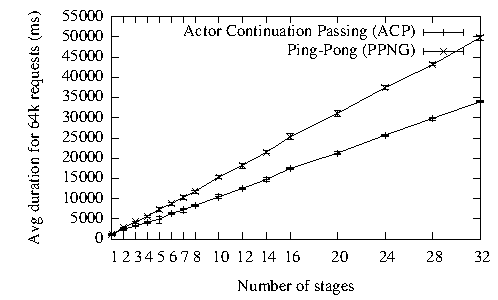
\includegraphics[width=.33\hsize]{plots/BENCHMARK-8CORE-2009-03-01-23:59-LIN.pdf}%
% 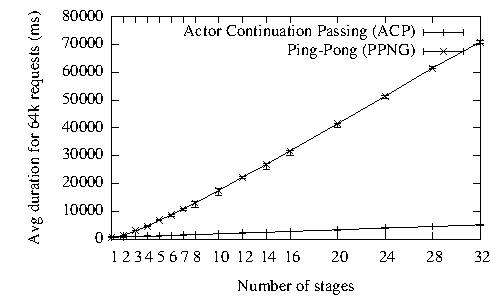
\includegraphics[width=.33\hsize]{plots/BENCHMARK-8CORE-2009-03-01-23:59-BLK.pdf}%
% 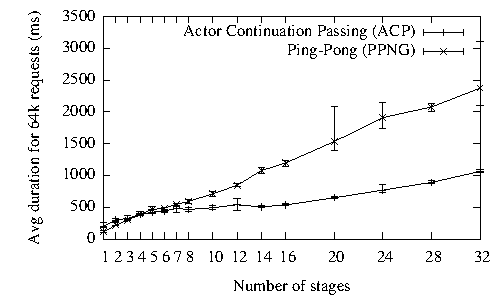
\includegraphics[width=.33\hsize]{plots/BENCHMARK-8CORE-2009-03-01-23:59-ALL.pdf}
% \end{center}
% \end{figure*}
	

\section{Implementation and Evaluation}
                                   

Soeuffleuse implements request handling according to the actor continuation passing approach on top
of the scala actor library. Stages are implemented as actors that run in separate
threads.\footnote{receive-actors in scala parlance} Their main loop listens for messages consisting
of one-argument anonymous lambda functions. When such a function is received, it is executed and
given access to the stage by passing the stage as its first argument. However, explicitely writing
out continuation functions can lead to unreadable source code with a nesting level of anonymous
lambda functions that is as large as the number of sequentially passed stages.

As a remedy, Souffleuse performs CPS-transform and sending of continuations at stage boundaries.
\emph{Continuation Passing Style (CPS)} refers to a control flow graph transformation that replaces
regular function return with calling a continuation function passed as an extra argument. Scala's
\textbf{for}-generator-expressions provide generator objects with continuation functions for the
remainer of the for-loop through a CPS-transform done by the scala compiler. How these continuatios
are called is left to the generator. This is exploited by Souffleuse's \textbf{goto} command to
capture the current continuation and send it to a remote stage for execution.

% Souffleuse currently does not support exception handling across stage boundaries and
% the DSL has no syntax support for non-sequential control-flows.


Souffleuse has been compared against using coordinator stages in a
messages-around-a-ring-of-stages-scenario with different load generation strategies. The results
indicate that it performs equally or better when the ring size is $\ge$~3. With growing ring size,
Soufflese converges towards a twofold performance increase since the required number of messages is
halved. The use of events consisting of serialized continuation functions appears to have neglible
overhead. All tests were conducted on a 8-core machine.


\section{Conclusion}

The results indicate that actor continuation passing is a viable approach for separating request
from stage logic without suffering from the performance penalty introduced by using explicit
coordinator stages. Souffleuse implements this approach as a mini-DSL in scala. The implementation
eliminates the need for deeply nested callbacks by using the implicit CPS-transformation of scala's
\textbf{for}-expression. Thus writing request logic as fast and concise request scripts is enabled,
while stage logic is implemented separately where it belongs.

\subsubsection*{Acknowledgments}

The author thanks Bj\"orn Kolbeck who initially described the problem in the context of XtreemFS,
a distributed filesystem implemented as a staged architecture.
           
\bibliographystyle{abbrv}
\bibliography{sigproc}  

\end{document}
